\section{Results}
\label{sec:results}

\begin{table*}[pos=t]
\centering
\setlength{\tabcolsep}{3pt}
\renewcommand{\arraystretch}{1.08}
% terracotta = positive / high, blue = negative / low, sage = magnitude of Read and Ans; darker = larger magnitude
\definecolor{cfSage1}{HTML}{ECF3EF}
\definecolor{cfSage2}{HTML}{D5E5DB}
\definecolor{cfSage3}{HTML}{B9D4C3}
\definecolor{cfSage4}{HTML}{9EC3AC}
\definecolor{cfSlate1}{HTML}{EAF0F6}
\definecolor{cfSlate2}{HTML}{D0DDEA}
\definecolor{cfSlate3}{HTML}{B1C7DD}
\definecolor{cfSlate4}{HTML}{94B2D0}
\definecolor{cfTerra1}{HTML}{F7ECEA}
\definecolor{cfTerra2}{HTML}{EED5D1}
\definecolor{cfTerra3}{HTML}{E2B8B2}
\definecolor{cfTerra4}{HTML}{D79E95}
\definecolor{cfOat1}{HTML}{F4EFE6}
\definecolor{cfOat2}{HTML}{E8DDC8}
\definecolor{cfGrey}{HTML}{E4E1DC}

\caption{\textbf{RAW grades by checkpoint and dataset.} Read, Ans, and Own give mean probe selectivity, clean-answer AUROC, and row margin. Superscripts count concepts meeting each grade. The final columns give the owned share for chest radiographs and COCO and their ratio. Blue indicates a negative row margin.}
\label{tab:cf-main}
\fitwidth{%
\cftabsize
\begin{tabular}{l@{\hspace{7pt}}ccc@{\hspace{4pt}}ccc@{\hspace{4pt}}ccc@{\hspace{4pt}}ccc}
\toprule
\multirow{2}{*}{Checkpoint} & \multicolumn{3}{c}{NIH ChestX-ray14} & \multicolumn{3}{c}{CheXpert Plus} & \multicolumn{3}{c}{COCO (control)} & \multicolumn{3}{c}{Owned share}\\
\cmidrule(lr){2-4}\cmidrule(lr){5-7}\cmidrule(lr){8-10}\cmidrule(lr){11-13}
& \multicolumn{1}{c}{Read} & \multicolumn{1}{c}{Ans} & \multicolumn{1}{c}{Own} & \multicolumn{1}{c}{Read} & \multicolumn{1}{c}{Ans} & \multicolumn{1}{c}{Own} & \multicolumn{1}{c}{Read} & \multicolumn{1}{c}{Ans} & \multicolumn{1}{c}{Own} & \multicolumn{1}{c}{clin.} & \multicolumn{1}{c}{COCO} & \multicolumn{1}{c}{ratio}\\
\midrule
Lingshu 32B & \cellcolor{cfSage2}0.08$^{5}$ & \cellcolor{cfSage3}0.78$^{6}$ & \cellcolor{cfSlate2}-0.02$^{2}$ & \cellcolor{cfSage4}0.20$^{5}$ & \cellcolor{cfSage3}0.87$^{5}$ & \cellcolor{cfTerra2}+0.04$^{5}$ & \cellcolor{cfSage1}0.03$^{4}$ & \cellcolor{cfSage4}0.95$^{5}$ & \cellcolor{cfTerra4}+0.28$^{6}$ & \cellcolor{cfTerra4}58\% & \cellcolor{cfTerra4}100\% & 58\% \\
CheXagent-2-3B & \cellcolor{cfSage3}0.13$^{5}$ & \cellcolor{cfSage3}0.86$^{6}$ & \cellcolor{cfTerra1}+0.00$^{2}$ & \cellcolor{cfSage4}0.21$^{5}$ & \cellcolor{cfSage4}0.95$^{5}$ & \cellcolor{cfTerra1}+0.01$^{4}$ & \cellcolor{cfSage3}0.13$^{5}$ & \cellcolor{cfSage3}0.81$^{5}$ & \cellcolor{cfTerra2}+0.03$^{2}$ & \cellcolor{cfTerra4}50\% & \cellcolor{cfTerra2}33\% & 150\% \\
Lingshu 7B & \cellcolor{cfSage2}0.08$^{5}$ & \cellcolor{cfSage3}0.76$^{6}$ & \cellcolor{cfTerra2}+0.02$^{1}$ & \cellcolor{cfSage4}0.21$^{4}$ & \cellcolor{cfSage3}0.86$^{5}$ & \cellcolor{cfTerra2}+0.04$^{4}$ & \cellcolor{cfSage1}0.02$^{4}$ & \cellcolor{cfSage4}0.97$^{5}$ & \cellcolor{cfTerra4}+0.68$^{6}$ & \cellcolor{cfTerra4}42\% & \cellcolor{cfTerra4}100\% & 42\% \\
Qwen2.5-VL-72B & \cellcolor{cfSage2}0.07$^{5}$ & \cellcolor{cfSage2}0.62$^{5}$ & \cellcolor{cfSlate2}-0.03$^{3}$ & \cellcolor{cfSage3}0.20$^{5}$ & \cellcolor{cfSage2}0.71$^{5}$ & \cellcolor{cfSlate2}-0.09$^{1}$ & \cellcolor{cfSage1}0.01$^{3}$ & \cellcolor{cfSage4}0.99$^{5}$ & \cellcolor{cfTerra4}+0.66$^{6}$ & \cellcolor{cfTerra3}33\% & \cellcolor{cfTerra4}100\% & 33\% \\
Qwen3-VL-32B & \cellcolor{cfSage2}0.10$^{5}$ & \cellcolor{cfSage2}0.70$^{6}$ & \cellcolor{cfSlate2}-0.02$^{2}$ & \cellcolor{cfSage3}0.17$^{5}$ & \cellcolor{cfSage3}0.82$^{5}$ & \cellcolor{cfSlate2}-0.02$^{2}$ & \cellcolor{cfSage2}0.05$^{4}$ & \cellcolor{cfSage4}0.99$^{5}$ & \cellcolor{cfTerra3}+0.15$^{6}$ & \cellcolor{cfTerra3}33\% & \cellcolor{cfTerra4}100\% & 33\% \\
InternVL3.5-38B & \cellcolor{cfSage2}0.10$^{5}$ & \cellcolor{cfSage3}0.78$^{6}$ & \cellcolor{cfSlate1}-0.00$^{1}$ & \cellcolor{cfSage3}0.17$^{5}$ & \cellcolor{cfSage3}0.86$^{5}$ & \cellcolor{cfSlate1}-0.00$^{2}$ & \cellcolor{cfSage2}0.08$^{5}$ & \cellcolor{cfSage4}0.99$^{5}$ & \cellcolor{cfTerra1}+0.01$^{6}$ & \cellcolor{cfTerra3}25\% & \cellcolor{cfTerra4}100\% & 25\% \\
Qwen3-VL-4B & \cellcolor{cfSage2}0.08$^{5}$ & \cellcolor{cfSage2}0.71$^{6}$ & \cellcolor{cfSlate3}-0.11$^{0}$ & \cellcolor{cfSage4}0.20$^{5}$ & \cellcolor{cfSage2}0.74$^{4}$ & \cellcolor{cfSlate1}-0.01$^{2}$ & \cellcolor{cfSage1}0.04$^{5}$ & \cellcolor{cfSage4}0.99$^{5}$ & \cellcolor{cfTerra4}+0.34$^{6}$ & \cellcolor{cfTerra3}17\% & \cellcolor{cfTerra4}100\% & 17\% \\
InternVL3.5-14B & \cellcolor{cfSage2}0.07$^{5}$ & \cellcolor{cfSage2}0.73$^{6}$ & \cellcolor{cfSlate1}-0.00$^{1}$ & \cellcolor{cfSage3}0.16$^{4}$ & \cellcolor{cfSage3}0.87$^{5}$ & \cellcolor{cfTerra1}+0.00$^{1}$ & \cellcolor{cfSage3}0.12$^{5}$ & \cellcolor{cfSage4}0.98$^{5}$ & \cellcolor{cfTerra1}+0.02$^{6}$ & \cellcolor{cfTerra3}17\% & \cellcolor{cfTerra4}100\% & 17\% \\
Gemma 3 12B & \cellcolor{cfSage2}0.07$^{5}$ & \cellcolor{cfSage2}0.62$^{6}$ & \cellcolor{cfSlate4}-0.37$^{1}$ & \cellcolor{cfSage3}0.18$^{5}$ & \cellcolor{cfSage1}0.52$^{4}$ & \cellcolor{cfSlate4}-0.38$^{1}$ & \cellcolor{cfSage2}0.07$^{5}$ & \cellcolor{cfSage4}0.95$^{5}$ & \cellcolor{cfTerra4}+0.44$^{6}$ & \cellcolor{cfTerra3}17\% & \cellcolor{cfTerra4}100\% & 17\% \\
Gemma 3 27B & \cellcolor{cfSage2}0.07$^{5}$ & \cellcolor{cfSage2}0.60$^{6}$ & \cellcolor{cfSlate2}-0.03$^{1}$ & \cellcolor{cfSage3}0.18$^{5}$ & \cellcolor{cfSage1}0.55$^{4}$ & \cellcolor{cfSlate1}-0.01$^{1}$ & \cellcolor{cfSage2}0.07$^{5}$ & \cellcolor{cfSage4}0.96$^{5}$ & \cellcolor{cfTerra4}+0.31$^{6}$ & \cellcolor{cfTerra3}17\% & \cellcolor{cfTerra4}100\% & 17\% \\
MedGemma 4B & \cellcolor{cfSage3}0.12$^{6}$ & \cellcolor{cfSage3}0.80$^{6}$ & \cellcolor{cfSlate3}-0.13$^{0}$ & \cellcolor{cfSage4}0.21$^{5}$ & \cellcolor{cfSage3}0.87$^{5}$ & \cellcolor{cfSlate3}-0.16$^{2}$ & \cellcolor{cfSage2}0.06$^{5}$ & \cellcolor{cfSage4}0.94$^{5}$ & \cellcolor{cfTerra3}+0.23$^{6}$ & \cellcolor{cfTerra3}17\% & \cellcolor{cfTerra4}100\% & 17\% \\
Qwen2.5-VL-32B & \cellcolor{cfSage2}0.09$^{6}$ & \cellcolor{cfSage2}0.63$^{5}$ & \cellcolor{cfSlate2}-0.06$^{1}$ & \cellcolor{cfSage3}0.16$^{5}$ & \cellcolor{cfSage2}0.70$^{5}$ & \cellcolor{cfSlate3}-0.11$^{0}$ & \cellcolor{cfSage1}0.02$^{4}$ & \cellcolor{cfSage4}0.99$^{5}$ & \cellcolor{cfTerra4}+0.38$^{6}$ & \cellcolor{cfTerra2}8\% & \cellcolor{cfTerra4}100\% & 8\% \\
InternVL3.5-8B & \cellcolor{cfSage2}0.06$^{5}$ & \cellcolor{cfSage2}0.73$^{6}$ & \cellcolor{cfSlate1}-0.01$^{0}$ & \cellcolor{cfSage3}0.19$^{4}$ & \cellcolor{cfSage3}0.86$^{5}$ & \cellcolor{cfSlate1}-0.00$^{1}$ & \cellcolor{cfSage2}0.12$^{5}$ & \cellcolor{cfSage4}0.98$^{5}$ & \cellcolor{cfTerra2}+0.03$^{6}$ & \cellcolor{cfTerra2}8\% & \cellcolor{cfTerra4}100\% & 8\% \\
HuatuoGPT-Vision-7B & \cellcolor{cfSage2}0.08$^{6}$ & \cellcolor{cfSage2}0.71$^{6}$ & \cellcolor{cfSlate2}-0.03$^{1}$ & \cellcolor{cfSage3}0.19$^{5}$ & \cellcolor{cfSage3}0.78$^{5}$ & \cellcolor{cfSlate1}-0.01$^{0}$ & \cellcolor{cfSage2}0.07$^{5}$ & \cellcolor{cfSage4}0.99$^{5}$ & \cellcolor{cfTerra1}+0.01$^{6}$ & \cellcolor{cfTerra2}8\% & \cellcolor{cfTerra4}100\% & 8\% \\
LLaVA-Med 1.5 7B & \cellcolor{cfSage2}0.08$^{6}$ & \cellcolor{cfSage1}0.53$^{5}$ & \cellcolor{cfSlate1}-0.01$^{0}$ & \cellcolor{cfSage3}0.19$^{5}$ & \cellcolor{cfSage1}0.59$^{5}$ & \cellcolor{cfSlate1}-0.01$^{1}$ & \cellcolor{cfSage2}0.07$^{5}$ & \cellcolor{cfSage3}0.76$^{5}$ & \cellcolor{cfTerra1}+0.00$^{1}$ & \cellcolor{cfTerra2}8\% & \cellcolor{cfTerra2}17\% & 50\% \\
CheXagent-8B & \cellcolor{cfSage3}0.16$^{6}$ & \cellcolor{cfSage2}0.73$^{6}$ & \cellcolor{cfSlate1}-0.00$^{0}$ & \cellcolor{cfSage4}0.23$^{5}$ & \cellcolor{cfSage3}0.88$^{5}$ & \cellcolor{cfSlate1}-0.02$^{1}$ & \cellcolor{cfSage2}0.05$^{5}$ & \cellcolor{cfSage1}0.52$^{3}$ & \cellcolor{cfSlate2}-0.03$^{0}$ & \cellcolor{cfTerra2}8\% & \cellcolor{cfTerra1}0\% & -- \\
Qwen2.5-VL-3B & \cellcolor{cfSage2}0.07$^{5}$ & \cellcolor{cfSage1}0.58$^{5}$ & \cellcolor{cfSlate2}-0.08$^{0}$ & \cellcolor{cfSage3}0.17$^{5}$ & \cellcolor{cfSage1}0.57$^{4}$ & \cellcolor{cfSlate2}-0.07$^{0}$ & \cellcolor{cfSage1}0.05$^{5}$ & \cellcolor{cfSage4}0.97$^{5}$ & \cellcolor{cfTerra4}+0.52$^{6}$ & \cellcolor{cfTerra1}0\% & \cellcolor{cfTerra4}100\% & 0\% \\
Qwen2.5-VL-7B & \cellcolor{cfSage2}0.08$^{5}$ & \cellcolor{cfSage2}0.62$^{6}$ & \cellcolor{cfSlate3}-0.14$^{0}$ & \cellcolor{cfSage3}0.20$^{4}$ & \cellcolor{cfSage2}0.65$^{5}$ & \cellcolor{cfSlate2}-0.08$^{0}$ & \cellcolor{cfSage1}0.02$^{4}$ & \cellcolor{cfSage4}0.98$^{5}$ & \cellcolor{cfTerra4}+0.67$^{6}$ & \cellcolor{cfTerra1}0\% & \cellcolor{cfTerra4}100\% & 0\% \\
Qwen3-VL-8B & \cellcolor{cfSage2}0.10$^{5}$ & \cellcolor{cfSage2}0.69$^{6}$ & \cellcolor{cfSlate1}-0.01$^{0}$ & \cellcolor{cfSage3}0.17$^{5}$ & \cellcolor{cfSage2}0.75$^{4}$ & \cellcolor{cfSlate2}-0.04$^{0}$ & \cellcolor{cfSage1}0.04$^{5}$ & \cellcolor{cfSage4}0.99$^{5}$ & \cellcolor{cfTerra4}+0.58$^{6}$ & \cellcolor{cfTerra1}0\% & \cellcolor{cfTerra4}100\% & 0\% \\
Gemma 3 4B & \cellcolor{cfSage2}0.07$^{5}$ & \cellcolor{cfSage1}0.56$^{5}$ & \cellcolor{cfSlate3}-0.11$^{0}$ & \cellcolor{cfSage3}0.18$^{5}$ & \cellcolor{cfSage1}0.53$^{3}$ & \cellcolor{cfSlate4}-0.27$^{0}$ & \cellcolor{cfSage2}0.07$^{5}$ & \cellcolor{cfSage4}0.94$^{5}$ & \cellcolor{cfTerra3}+0.24$^{5}$ & \cellcolor{cfTerra1}0\% & \cellcolor{cfTerra3}83\% & 0\% \\
LLaVA-1.5-7B & \cellcolor{cfSage2}0.08$^{6}$ & \cellcolor{cfSage1}0.51$^{5}$ & \cellcolor{cfSlate2}-0.04$^{0}$ & \cellcolor{cfSage3}0.17$^{5}$ & \cellcolor{cfSage1}0.52$^{3}$ & \cellcolor{cfSlate2}-0.03$^{0}$ & \cellcolor{cfSage4}0.28$^{5}$ & \cellcolor{cfSage4}0.97$^{5}$ & \cellcolor{cfTerra2}+0.03$^{5}$ & \cellcolor{cfTerra1}0\% & \cellcolor{cfTerra3}83\% & 0\% \\
MedGemma 27B & \cellcolor{cfSage3}0.12$^{6}$ & \cellcolor{cfSage3}0.80$^{6}$ & \cellcolor{cfSlate3}-0.14$^{0}$ & \cellcolor{cfSage4}0.21$^{5}$ & \cellcolor{cfSage3}0.87$^{5}$ & \cellcolor{cfSlate2}-0.06$^{0}$ & \cellcolor{cfSage2}0.06$^{5}$ & \cellcolor{cfSage4}0.97$^{5}$ & \cellcolor{cfTerra3}+0.12$^{4}$ & \cellcolor{cfTerra1}0\% & \cellcolor{cfTerra3}67\% & 0\% \\
LLaVA-1.5-13B & \cellcolor{cfSage2}0.08$^{6}$ & \cellcolor{cfSage1}0.53$^{5}$ & \cellcolor{cfSlate2}-0.02$^{0}$ & \cellcolor{cfSage3}0.17$^{5}$ & \cellcolor{cfSage1}0.51$^{3}$ & \cellcolor{cfSlate1}-0.01$^{0}$ & \cellcolor{cfSage4}0.28$^{5}$ & \cellcolor{cfSage4}0.96$^{5}$ & \cellcolor{cfTerra2}+0.02$^{3}$ & \cellcolor{cfTerra1}0\% & \cellcolor{cfTerra3}50\% & 0\% \\
Llama 3.2 Vision 11B & \cellcolor{cfSage2}0.08$^{6}$ & \cellcolor{cfSage2}0.65$^{6}$ & \cellcolor{cfSlate2}-0.03$^{0}$ & \cellcolor{cfSage3}0.16$^{5}$ & \cellcolor{cfSage2}0.73$^{5}$ & \cellcolor{cfSlate2}-0.04$^{0}$ & \cellcolor{cfSage3}0.12$^{5}$ & \cellcolor{cfSage4}0.95$^{5}$ & \cellcolor{cfSlate1}-0.01$^{1}$ & \cellcolor{cfTerra1}0\% & \cellcolor{cfTerra2}17\% & 0\% \\
LLaVA-Rad-7B & \cellcolor{cfSage3}0.15$^{6}$ & \cellcolor{cfSage2}0.71$^{6}$ & \cellcolor{cfSlate1}-0.01$^{0}$ & \cellcolor{cfSage4}0.27$^{5}$ & \cellcolor{cfSage3}0.87$^{5}$ & \cellcolor{cfSlate1}-0.02$^{0}$ & \cellcolor{cfSage3}0.12$^{5}$ & \cellcolor{cfSage1}0.50$^{3}$ & \cellcolor{cfSlate2}-0.03$^{0}$ & \cellcolor{cfTerra1}0\% & \cellcolor{cfTerra1}0\% & -- \\
\midrule
\textbf{All cells} & 0.09 & 0.68 & -0.06 & 0.19 & 0.74 & -0.05 & 0.08 & 0.92 & +0.23 & 15\% & 78\% & 19\% \\
\quad count / cells & 135/150 & 143/150 & 16/150 & 121/150 & 114/150 & 28/150 & 118/150 & 121/150 & 117/150 & & & \\
\bottomrule
\end{tabular}}
\end{table*}


\begin{figure*}[pos=t]
    \centering
    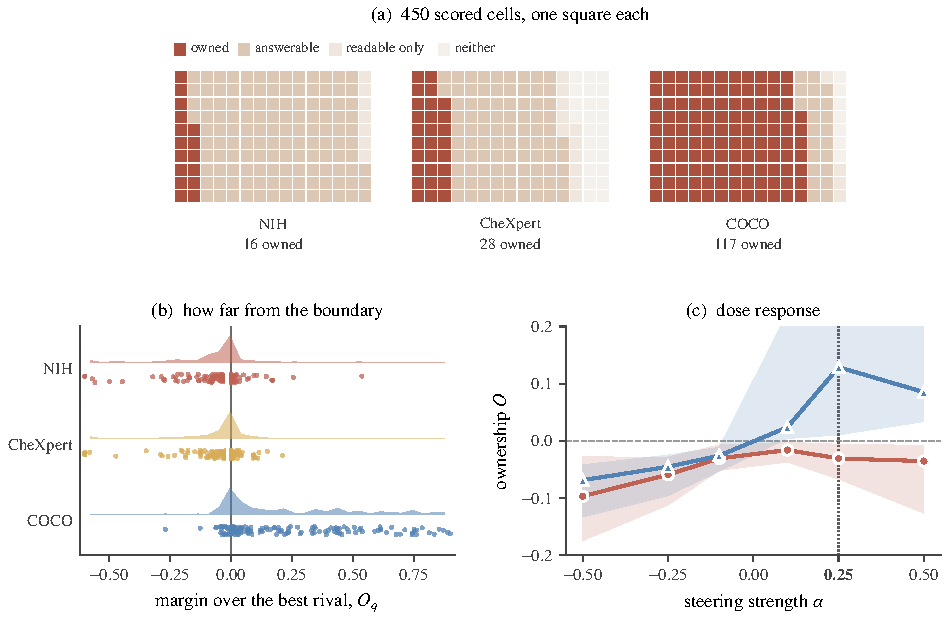
\includegraphics[width=\linewidth]{figures/fig2_overview.pdf}
    \caption{\textbf{Ownership margins by dataset and steering strength.} (a) Distribution of the row margin $O_q$ across checkpoint--concept pairs. (b) Median and interquartile range of $O_q$ by steering strength. The dotted line marks the primary strength.}
    \label{fig:overview}
\end{figure*}

\subsection{Decoding, answering, and control}
\label{sec:headline}

On the two chest datasets, \cfChestReadablePct{}\% of the \cfChestCellsN{} cells were readable and \cfChestAnswerablePct{}\% were answerable. Ownership was less common, at \cfChestOwnedPct{}\% on radiographs and \cfCocoOwnedPct{}\% on COCO (Table~\ref{tab:cf-main}, Fig.~\ref{fig:teaser}). Among the \cfReadAns{} chest cells that passed both reading and answering, only \cfReadAnsOwned{} were owned (\cfReadAnsOwnedPct{}\%). Across steering strengths, the median NIH ownership margin remained negative, while COCO had a positive median at the primary strength (Fig.~\ref{fig:overview}).

\subsection{What the competitor comparison adds}
\label{sec:deficit}

\begin{table}[pos=t]
\centering
\caption{\textbf{Ownership and direction specificity.} Counts of checkpoint--concept pairs. Each of the last three columns requires the steering reference to be met.}
\label{tab:specificity}
\small
\setlength{\tabcolsep}{3pt}
\begin{tabular}{@{}lrrrr@{}}
\toprule
Dataset & \shortstack{Reference\\met} & \shortstack{Owned\\(row)} &
\shortstack{Specific\\(column)} & \shortstack{Owned and\\specific} \\
\midrule
NIH & \jnRefNih & \jnOwnedNih & \jnColSpecNih & \jnTwoWayNih \\
CheXpert Plus & \jnRefChex & \jnOwnedChex & \jnColSpecChex & \jnTwoWayChex \\
Chest total & \jnRefChest & \jnOwnedChest & \jnColSpecChest & \jnTwoWayChest \\
COCO & \jnRefCoco & \jnOwnedCoco & \jnColSpecCoco & \jnTwoWayCoco \\
\bottomrule
\end{tabular}
\end{table}

On chest radiographs, \cfChestRefBelow{} of \cfChestCellsN{} label directions failed the random and sham reference. The median own effect was \cfMedianWqqNih{} on NIH and \cfMedianWqqChex{} on CheXpert Plus, compared with \cfMedianWqqCoco{} on COCO (Table~\ref{tab:cf-controls}). Across checkpoints, the intended question received \cfOwnShareNih{}\% of the total positive change on NIH and \cfOwnShareChex{}\% on CheXpert Plus, compared with \cfOwnShareCoco{}\% on COCO (Appendix~\ref{app:cf-figures}). The write matrices show that some directions raise several chest answers by similar amounts, while COCO effects tend to concentrate on the intended question (Fig.~\ref{fig:write-matrices}).

The reference alone would certify \jnRefChest{} of \cfChestCellsN{} chest directions. Requiring each direction to win on its own question excluded \jnRefLostChest{}. Requiring it also to affect its own answer more than every other answer excluded \jnOwnedNotColChest{} of the \cfChestOwned{} remaining directions. Thus \jnRefNotTwoWayChest{} of the \jnRefChest{} chest directions that passed the reference (\jnRefNotTwoWayChestPct{}\%) failed at least one of the two concept comparisons. On COCO, every direction that met the reference also passed the row comparison, and \jnOwnedNotColCoco{} of \jnRefCoco{} (\jnRefNotTwoWayCocoPct{}\%) failed the column comparison. Overall, \jnTwoWayChest{} of \cfChestCellsN{} chest cells (\jnTwoWayChestPct{}\%) were owned and specific, comprising \jnTwoWayNih{} of \cfNihCells{} on NIH and \jnTwoWayChex{} of \cfChexCells{} on CheXpert Plus. On COCO, \jnTwoWayCoco{} of \cfCocoCells{} (\jnTwoWayCocoPct{}\%) passed both comparisons (Table~\ref{tab:specificity}).

Among directions that met the steering reference, the sum of absolute changes across the other five answers was a median of \jnOffTargetChest{} times the own effect on chest radiographs and \jnOffTargetCoco{} times on COCO. Across all directions, median column selectivity was \jnKappaMedChest{} on chest radiographs and \jnKappaMedCoco{} on COCO (Eq.~\ref{eq:column-selectivity}).

\begin{figure*}[pos=t]
    \centering
    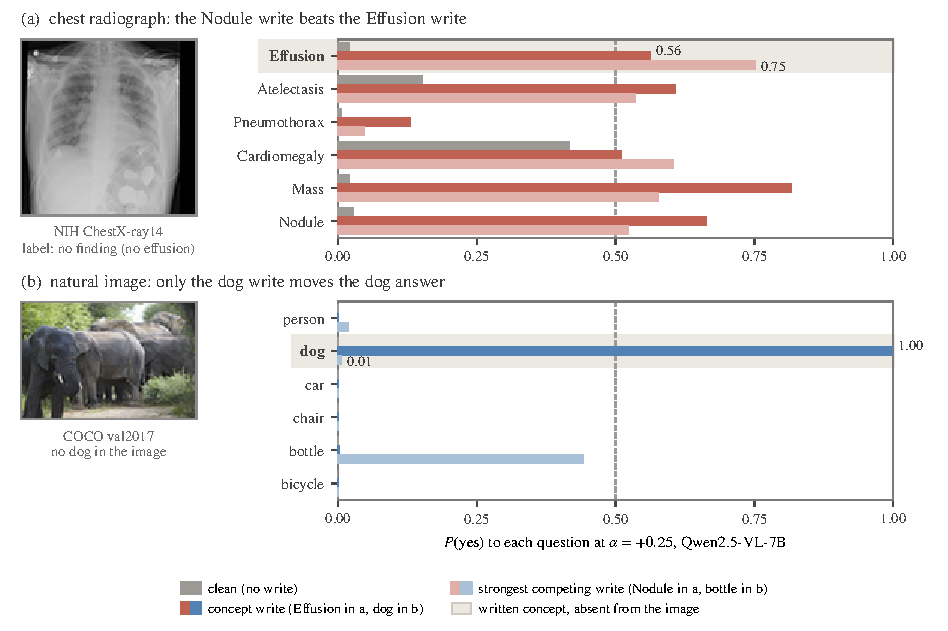
\includegraphics[width=\linewidth]{figures/fig3_example.pdf}
    \caption{\textbf{Answer changes on a radiograph and a photograph.} Qwen2.5-VL-7B's probability of answering yes to each question is shown before editing and after adding the target or strongest competing direction. Shading marks the target question. The dashed line marks equal support for yes and no.}
    \label{fig:example}
\end{figure*}

\label{sec:seed}
The effusion answer again moved more under the nodule write in an independent NIH test cohort ($O_{\mathrm{Effusion}}=\cfSeedEffO$; Table~\ref{tab:cf-seed}). Across chest blocks, \cfEffusionOwnedBlocks{} of \cfChestBlocks{} effusion answers were owned. On the radiograph in Fig.~\ref{fig:example}, the probability of a yes answer for effusion rose from \cfExChestClean{} to \cfExChestOwn{} with the effusion direction and to \cfExChestComp{} with the nodule direction. On the photograph, the dog direction raised the dog answer from \cfExCocoClean{} to \cfExCocoOwn{}, with negligible change in the other answers.

\subsection{Sensitivity to competitors and direction construction}
\label{sec:controls}
\label{sec:robust-geometry}

Averaging across all possible choices of one, two, three, and four competitors gave \jnSubOneChest{}, \jnSubTwoChest{}, \jnSubThreeChest{}, and \jnSubFourChest{} owned chest cells, respectively, compared with \cfChestOwned{} using all five. The COCO count stayed at \cfCocoOwned{} for every subset size. Even one randomly chosen competitor left a wide gap between the domains. The strongest competitor matched the most similar direction at about the chance rate, as it did the most frequently co-occurring label (Table~\ref{tab:cf-geometry}). Adding the other eligible labels to the chest competitor set retained \cfExtcompRetained{} of \cfExtcompOwned{} originally owned cells in the blocks tested.

In owned cells, ranks ranged from \jnOwnedRankMin{} to \jnOwnedRankMax{} when the label write was compared with its \jnRandomDirections{} random reference writes (Fig.~\ref{fig:rank}). Alternative directions fitted from class means, from the feature pattern associated with the probe, or after removing information shared with other concepts yielded ownership rates of \cfAltdirChestPctMin{}--\cfAltdirChestPctMax{}\% on the chest datasets and \cfAltdirCocoPctMin{}--\cfAltdirCocoPctMax{}\% on COCO (Table~\ref{tab:cf-altdir}). The ownership grade agreed with the original evaluation in \cfValidOwnedAgree{} of \cfValidCells{} cells when evaluated on a separate set of \cfValidRows{} CheXpert films with radiologist consensus labels. Refit directions trained on those labels were owned in \cfValidfitOwnedExpert{} of \cfValidfitCells{} cells, compared with \cfValidfitOwnedReport{} for directions trained on report labels. Repeating the probe fit preserved ownership on both refits in \cfRefitGradeStableNih{} of \cfRefitGradeOwnedNih{} owned NIH cells and \cfRefitGradeStableCoco{} of \cfRefitGradeOwnedCoco{} owned COCO cells (Table~\ref{tab:cf-refit}).

\subsection{Ownership at comparable answer difficulty}
\label{sec:coco}

Across checkpoints tested with both sets of COCO categories, the fine-grained objects had a lower median clean-answer AUROC than the common objects (\cfFgFineAuroc{} versus \cfFgEasySameAuroc{}). Fine-grained objects were owned in \cfFgFineOwned{} of \cfFgFineCells{} cells, compared with \cfFgEasySameOwned{} of \cfFgEasySameCells{} for common objects (Appendix~\ref{app:cf-difficulty}). In the highest AUROC stratum (AUROC $\geq\cfStratTopEdge$), \cfStratChestTopOwned{} of \cfStratChestTopN{} chest cells were owned, compared with \cfStratNatTopOwned{} of \cfStratNatTopN{} natural-image cells. The chest-minus-natural difference was \jnTopDiff{} (bootstrap standard deviation \jnTopDiffSd{}). Most chest cells in that stratum came from CheXpert Plus.

The lower common-support cutoff included \jnCsEightyChestN{} chest cells, of which \jnCsEightyChestOwned{} (\jnCsEightyChestPct{}\%) were owned, and \jnCsEightyNatN{} natural-image cells, of which \jnCsEightyNatOwned{} (\jnCsEightyNatPct{}\%) were owned. NIH contributed \jnCsEightyNihN{} of the chest cells and \jnCsEightyNihOwned{} owned cells. After adjustment for clean-answer AUROC and probe selectivity, the chest-minus-natural difference in ownership probability was \jnCsEightyAdj{} (bootstrap standard deviation \jnCsEightyAdjSd{}). At the higher cutoff, the adjusted difference was \jnCsEightyFiveAdj{} (bootstrap standard deviation \jnCsEightyFiveAdjSd{}).

\subsection{Non-clinical attributes of the same radiographs}
\label{sec:attributes}

The probes distinguished projection, recorded sex, and age at least as well as clinical findings on the same radiographs. Median probe AUROC was \cfAttrAurocMin{}--\cfAttrAurocMax{} for the attributes and \cfAttrClinAuroc{} for findings (Appendix~\ref{app:cf-attributes}). With both types of direction included in the comparison, \cfAttrAllAttrOwned{} of \cfAttrAllAttrN{} attribute cells were owned, as were \cfAttrAllClinOwned{} of \cfAttrAllClinN{} finding cells. In the highest clean-answer AUROC stratum of this comparison, \cfStratAttrTopOwned{} of \cfStratAttrTopN{} attribute cells and \cfStratFindTopOwned{} of \cfStratFindTopN{} finding cells were owned.

\subsection{Effects of the components downstream of the vision tower}
\label{sec:reader}

Checkpoints that shared a vision tower and used the same directions differed in which answers those directions controlled (Fig.~\ref{fig:readers}). Ownership margins differed by more than the typical variation across probe refits in \cfPairsRatioAboveOne{} of \cfPairsRatioN{} shared-tower comparisons (Table~\ref{tab:cf-pairs}). The differences persisted when both readers received identical image features.

The crossed Gemma and MedGemma experiment exchanged the reader or the tower while holding the other component fixed. On NIH, the mean absolute change in $O_q$ was \cfSwapReaderNihOMin{} for a reader swap and \cfSwapTowerNihOMin{} for a tower swap. For $W_{q,q}$, the corresponding changes were \cfSwapReaderNihMin{} and \cfSwapTowerNihMin{}. On COCO, the tower swap had the larger effect on $O_q$ (\cfSwapTowerCocoOMin{} versus \cfSwapReaderCocoOMin{}). Across the \cfSwapCombos{} tower--reader combinations, \cfSwapChestOwned{} of \cfSwapChestCells{} chest cells were owned, compared with \cfSwapCocoOwned{} of \cfSwapCocoCells{} COCO cells (Appendix~\ref{app:cf-crossed-reader}).

When the write was applied after the connector, the median ownership margin remained negative on NIH and CheXpert Plus and positive on COCO (Table~\ref{tab:cf-controls}). At that site the edit bypassed the connector, and the language model alone reproduced the sign pattern. Models with chest-trained towers had a higher median NIH probe AUROC than the other checkpoints (\cfSpecTowerProbeAuroc{} versus \cfSpecRestProbeAuroc{}) and owned \cfSpecTowerOwned{} of \cfSpecTowerN{} chest cells. The effect of model size varied across families and findings (Fig.~\ref{fig:ladders}).

\subsection{Control of the model's answer}
\label{sec:ansdir}

The answer direction was owned in \cfAnsChestOwnedA{} of \cfAnsChestN{} chest cells, compared with \cfAnsChestOwnedLabel{} for the label direction (Table~\ref{tab:cf-ansdir}). Higher ownership was expected because we fitted this direction to the model's answers. The two directions were nearly perpendicular on chest radiographs, with a median cosine of \cfAnsCosChestMed{}, and aligned more closely on COCO, with a median cosine of \cfAnsCosCocoMed{}.

On chest radiographs, the answer direction gave a median AUROC of \cfValAurocAnsCleanChest{} against the model's clean answers and \cfValAurocAnsChest{} against the report labels. The label direction gave \cfValAurocProbeCleanChest{} and \cfValAurocProbeChest{}, respectively (Table~\ref{tab:cf-validation}). The answer direction changes the model's output along a signal with weaker agreement with the report labels. Its effect on output is evidence of answer control, and clinical interpretation would require agreement with independently established findings. The ownership advantage also appeared across the tests of negated questions, forced choices, and report continuations (\cfSemAnswerOwned{} of \cfSemCells{} cells for answer directions versus \cfSemLabelOwned{} for label directions; Table~\ref{tab:cf-semend}).

\FloatBarrier
